\documentclass{beamer}
\usepackage[utf8]{inputenc}
\usepackage[T1]{fontenc}
\usepackage{listings}

\usepackage{tikz}
\usetikzlibrary{shapes.geometric, arrows}

\tikzset{
  block/.style={
    rectangle,
    draw,
    draw=black,
    fill=gray!10,
    execute at begin node=\setlength{\baselineskip}{8pt}
  }
}
\tikzset{
  blockhighlight/.style={
    rectangle,
    draw,
    draw=black,
    fill=green!10,
    execute at begin node=\setlength{\baselineskip}{8pt}
  }
}

%\tikzstyle{block} = [rectangle, draw, draw=black, fill=gray!10, execute at begin node \setlength{\baselineskip}{4pt}]
\tikzstyle{arrow} = [->, > = latex']
\def\code#1{\scriptsize{\texttt{#1}}}

\lstset{basicstyle=\scriptsize\ttfamily,breaklines=true}
\lstset{framextopmargin=50pt}

\title{MAYHEM Sword Binary Introduction}
\date{\today}
\author[Eubanks]{Alex Eubanks \texttt{<alex.eubanks@forallsecure.com>}}

\usetheme{fas}

\begin{document}

\begin{frame}
\titlepage
\end{frame}

\section{Agenda}

\begin{frame}{Agenda}
\setlength{\parskip}{0cm}
\tableofcontents
\end{frame}

\section{Introduction}

\begin{frame}
\frametitle{Requirements}
\begin{itemize}
  \item A working copy of MAYHEM Sword.
  \item MAYHEM client installed on the command line in a modern linux distribution, such as Ubuntu or Debian.
\end{itemize}
\end{frame}

\begin{frame}
\frametitle{Basic Vocabulary}
\begin{itemize}
  \item \textbf{Corpus} - A set of inputs.
  \item \textbf{Harness} - A harness is a special-purpose program, created to better test code or another application.
  \item \textbf{Input} - Input refers to data generated by the fuzzer to run within a program. A program may read configuration files, or receive various user inputs, but within the context of fuzzing input refers only to the input generated by the fuzzer and used to test the program. The Input changes each time the fuzzer runs.
  \item \textbf{Invoke} - To run a program over a given input.
  \item \textbf{Program Under Test} - The Program Under Test is the program being tested by the fuzzer.
  \item \textbf{Program} - Program can refer to a Program Under Test, or harness, depending on context.
  \item \textbf{Test Case} - A synonym for input.
\end{itemize}
\end{frame}

\begin{frame}
\frametitle{What can MAYHEM Analyze?}
In order for our binary to be analyzed with MAYHEM, the following properties must hold:

\begin{itemize}
  \item The binary application must accept input through a means supported by MAYHEM.
  \item The binary application must run on an architecture and operating system supported by MAYHEM.
  \item You are looking for errors in the binary you are testing.
\end{itemize}
\end{frame}


\section{Understanding objdump}

\begin{frame}[fragile]
\frametitle{Packaging objdump}
\texttt{objdump} is an application distributed with GNU binutils to dump and display information about programs stored in common binary executable file formats. We will package \texttt{objdump} for MAYHEM, and upload \texttt{objdump} to our instance of MAYHEM Sword.

To begin, we will install \texttt{objdump}. To do this on a debian-based distro (Debian, Ubuntu, etc.), we run:

\begin{lstlisting}
   apt-get update && \
   apt-get upgrade -y && \
   apt-get install -y binutils
\end{lstlisting}
\end{frame}

\begin{frame}[fragile]
\frametitle{Running objdump}
We can now run \texttt{objdump}, and see what options are available.

\begin{lstlisting}[basicstyle=\tiny]
root@d5ec5618a4ed:~# objdump /bin/ls
Usage: objdump <option(s)> <file(s)>
 Display information from object <file(s)>.
 At least one of the following switches must be given:
  -a, --archive-headers    Display archive header information
  -f, --file-headers       Display the contents of the overall file header
  -p, --private-headers    Display object format specific file header contents
  -P, --private=OPT,OPT... Display object format specific contents
  -h, --[section-]headers  Display the contents of the section headers
  -x, --all-headers        Display the contents of all headers
...
  -r, --reloc              Display the relocation entries in the file
  -R, --dynamic-reloc      Display the dynamic relocation entries in the file
  @<file>                  Read options from <file>
  -v, --version            Display this program's version number
  -i, --info               List object formats and architectures supported
  -H, --help               Display this information
root@d5ec5618a4ed:~# 
\end{lstlisting}
\end{frame}

\begin{frame}[fragile]
\frametitle{objdump with flags}
Running with no flags isn't very helpful. If we take a look at the help menu that's printed out, we see there's a variety of flags printed out. The flags \texttt{-x} and \texttt{-s} look useful. Let's try running again with those flags.

\begin{lstlisting}[basicstyle=\tiny]
root@d5ec5618a4ed:~# objdump -xD /bin/ls | head

/bin/ls:     file format elf64-x86-64
/bin/ls
architecture: i386:x86-64, flags 0x00000150:
HAS_SYMS, DYNAMIC, D_PAGED
start address 0x0000000000005430

Program Header:
    PHDR off    0x0000000000000040 vaddr 0x0000000000000040 paddr 0x0000000000000040 align 2**3
         filesz 0x00000000000001f8 memsz 0x00000000000001f8 flags r-x
         
...
         
  1d:   35 62 64 31 30          xor    $0x30316462,%eax
  22:   65 63 63 64             movslq %gs:0x64(%rbx),%esp
  26:   2e 64 65 62             cs fs gs (bad) {%k6}
  2a:   75 67                   jne    93 <_init@@Base-0x3435>
  2c:   00 00                   add    %al,(%rax)
  2e:   00 00                   add    %al,(%rax)
  30:   c2 01 46                retq   $0x4601
  33:   f8                      clc    
root@d5ec5618a4ed:~# 
\end{lstlisting}
\end{frame}

\section{Packaging objdump}

\begin{frame}[fragile]
\frametitle{mayhem package objdump}
Terrific. Now we know exactly how we want to invoke \texttt{objdump}, with the \texttt{-xD} flags.

To package this binary, we run \texttt{mayhem package /usr/bin/objdump}. Let's try that out now.

\begin{lstlisting}[basicstyle=\tiny]
root@d5ec5618a4ed:~# mayhem package /usr/bin/objdump
INFO:root:Packaging application: /usr/bin/objdump
INFO:root:Packaging dependency: /usr/bin/objdump -> /tmp/objdump-wng7lsdf/root/usr/bin/objdump
INFO:root:Packaging dependency: /lib/x86_64-linux-gnu/libz.so.1 -> /tmp/objdump-wng7lsdf/root/lib/x86_64-linux-gnu/libz.so.1
INFO:root:Packaging dependency: /usr/lib/x86_64-linux-gnu/libopcodes-2.28-system.so -> /tmp/objdump-wng7lsdf/root/usr/lib/x86_64-linux-gnu/libopcodes-2.28-system.so
INFO:root:Packaging dependency: /usr/lib/x86_64-linux-gnu/libbfd-2.28-system.so -> /tmp/objdump-wng7lsdf/root/usr/lib/x86_64-linux-gnu/libbfd-2.28-system.so
INFO:root:Generating default configuration under: /tmp/objdump-wng7lsdf/config.json
INFO:root:Packaged /usr/bin/objdump under: /tmp/objdump-wng7lsdf
root@d5ec5618a4ed:~# 
\end{lstlisting}
\end{frame}

\begin{frame}[fragile]
\frametitle{Package directory contents}
There are a few files and folders inside the package we have created at \texttt{/tmp/objdump-wng7lsdf}.

\begin{lstlisting}[basicstyle=\tiny]
root@d5ec5618a4ed:~# ls -lh /tmp/objdump-wng7lsdf
total 12K
-rw-r--r-- 1 root root  277 Jul  9 20:45 config.json
drwxr-xr-x 2 root root 4.0K Jul  9 20:45 corpus
drwxr-xr-x 4 root root 4.0K Jul  9 20:45 root
\end{lstlisting}
\end{frame}

\begin{frame}[fragile]
\frametitle{The corpus directory}
The \texttt{corpus} directory contains seed inputs. Earlier, when we talked about mutation-based input generation, these are the inputs that MAYHEM would mutate. Fortunate for us, objdump parses linux executables, and we have plenty of those right in our example VM. Let's copy a couple over to the corpus directory.

\begin{lstlisting}[basicstyle=\tiny]
~# cp /bin/pwd /tmp/objdump-wng7lsdf/corpus/
~# cp /bin/true /tmp/objdump-wng7lsdf/corpus/
~# cp /bin/cat /tmp/objdump-wng7lsdf/corpus/
\end{lstlisting}

The root directory contains all of the files and dependencies required for MAYHEM to invoke and run the binary we wish to test. This directory has been auto-populated with the dynamically-linked runtime dependencies for us.
\end{frame}

\begin{frame}[fragile]
\frametitle{config.json}

The \texttt{config.json} file contains auto-populated configuration information for MAYHEM, informing MAYHEM how to invoke and run our binary under test.

We do need to modify the \texttt{config.json} file. Let's take a look at what's inside first.

\begin{lstlisting}[basicstyle=\tiny]
root@d5ec5618a4ed:~# cat /tmp/objdump-wng7lsdf/config.json 
{
    "fuzzers": [
        {
            "target_args": [
                "@@"
            ],
            "target_input": "@@",
            "library_path": "root/usr/lib/x86_64-linux-gnu:root/lib/x86_64-linux-gnu",
            "target": "root/usr/bin/objdump"
        }
    ]
}
\end{lstlisting}
\end{frame}

\begin{frame}[fragile]
\frametitle{Changing config.json}
For the purposes of this tutorial, we are only concerned with the \texttt{"target\_args"} field. This is a json array of command-line arguments to be passed to the target binary. \texttt{"@@"} is a special argument that tells MAYHEM, "Create an input filename for me, and place it here." We want to pass the command line argument \texttt{-xD} before \texttt{@@}, so we will change \texttt{"target\_args"} to look like this:

\begin{lstlisting}[basicstyle=\tiny]
            "target_args": [
                "-xD",
                ""@@"
            ]
\end{lstlisting}
\end{frame}

\section{Uploading the objdump Package}

\begin{frame}[fragile]
\frametitle{mayhem upload}
We're now going to upload this package to MAYHEM. We need the URL for the running instance of MAYHEM we wish to upload this package to. For me, this URL is \texttt{http://192.168.99.101:32434}.

To upload, I will type:

\begin{lstlisting}[basicstyle=\tiny]
    mayhem upload --start-sword -u http://192.168.99.101:32434/ /tmp/objdump-wng7lsdf
\end{lstlisting}

\texttt{--start-sword} tells MAYHEM to start fuzzing as soon as the binary is uploaded, and \texttt{-u} allows us to specify a URL to our specific instance of MAYHEM.
\end{frame}

\begin{frame}
\frametitle{MAYHEM Sword Running}
  \begin{tikzpicture}
  \node[inner sep=0pt]
    {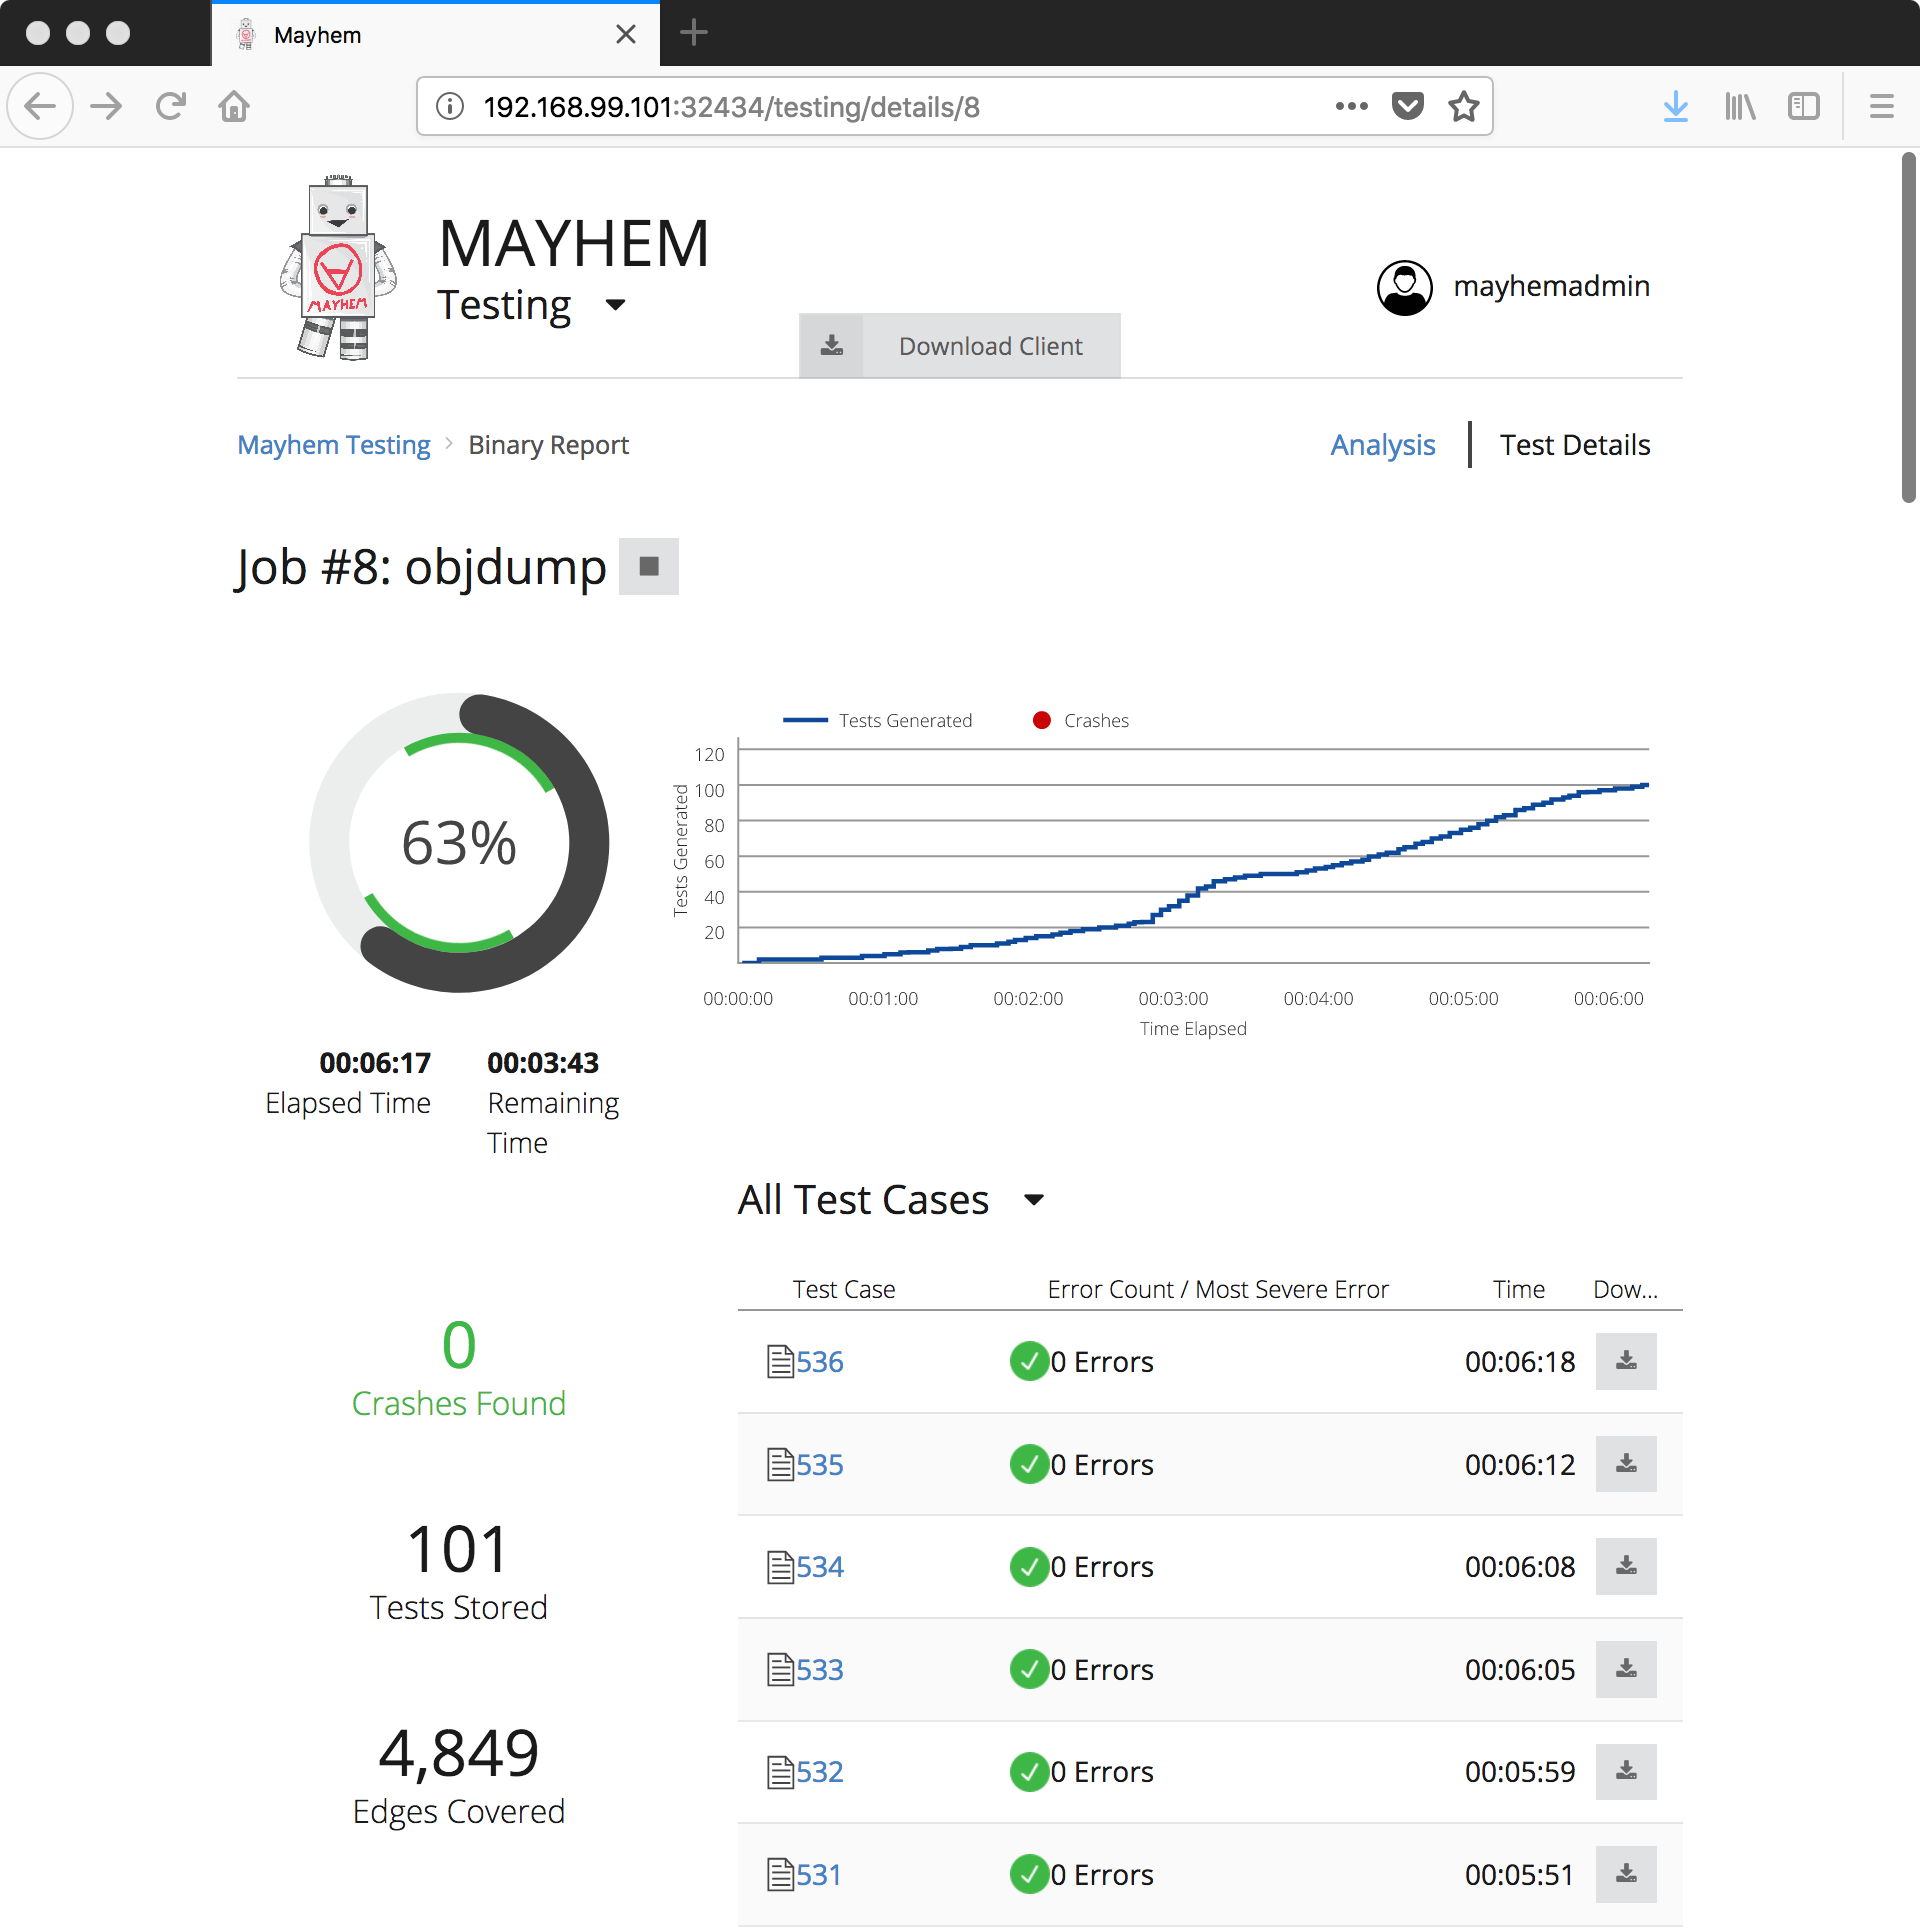
\includegraphics[width=1\textwidth]{images/mayhem-gui-screenshot.png}};
  \end{tikzpicture}
\end{frame}

\end{document}